%
% $RCSfile: placement.tex,v $
%
% Copyright (C) 2002-2008. Christian Heller.
%
% Permission is granted to copy, distribute and/or modify this document
% under the terms of the GNU Free Documentation License, Version 1.1 or
% any later version published by the Free Software Foundation; with no
% Invariant Sections, with no Front-Cover Texts and with no Back-Cover
% Texts. A copy of the license is included in the section entitled
% "GNU Free Documentation License".
%
% http://www.cybop.net
% - Cybernetics Oriented Programming -
%
% http://www.resmedicinae.org
% - Information in Medicine -
%
% Version: $Revision: 1.1 $ $Date: 2008-08-19 20:41:08 $ $Author: christian $
% Authors: Christian Heller <christian.heller@tuxtax.de>
%

\subsection{Placement}
\label{placement_heading}
\index{Layered Architecture}
\index{Communication Patterns placed in Layered Architecture}
\index{Model View Controller Pattern}
\index{MVC}
\index{Presentation Layer}
\index{Data Mapper Pattern}
\index{Entity Relationship Model}
\index{ERM}
\index{Database}
\index{DB}
\index{Data Transfer Object}
\index{DTO}
\index{Assembler}

Many state-of-the-art software systems consist of a layered architecture
similar to the one shown in figure \ref{logical_figure}. Yet how do the
communication patterns explained before suit this classical architecture? In
the traditional model of a layered software system, a startable process, best
placed in the \emph{Controller}, creates the whole application tree, to which
belong the \emph{Views} (as user interface), several \emph{Models} of the
\emph{Domain} (providing data to the views and as facade to remote servers) and
the \emph{Data Mapper} (translating between domain- and database model).

\begin{figure}[ht]
    \begin{center}
        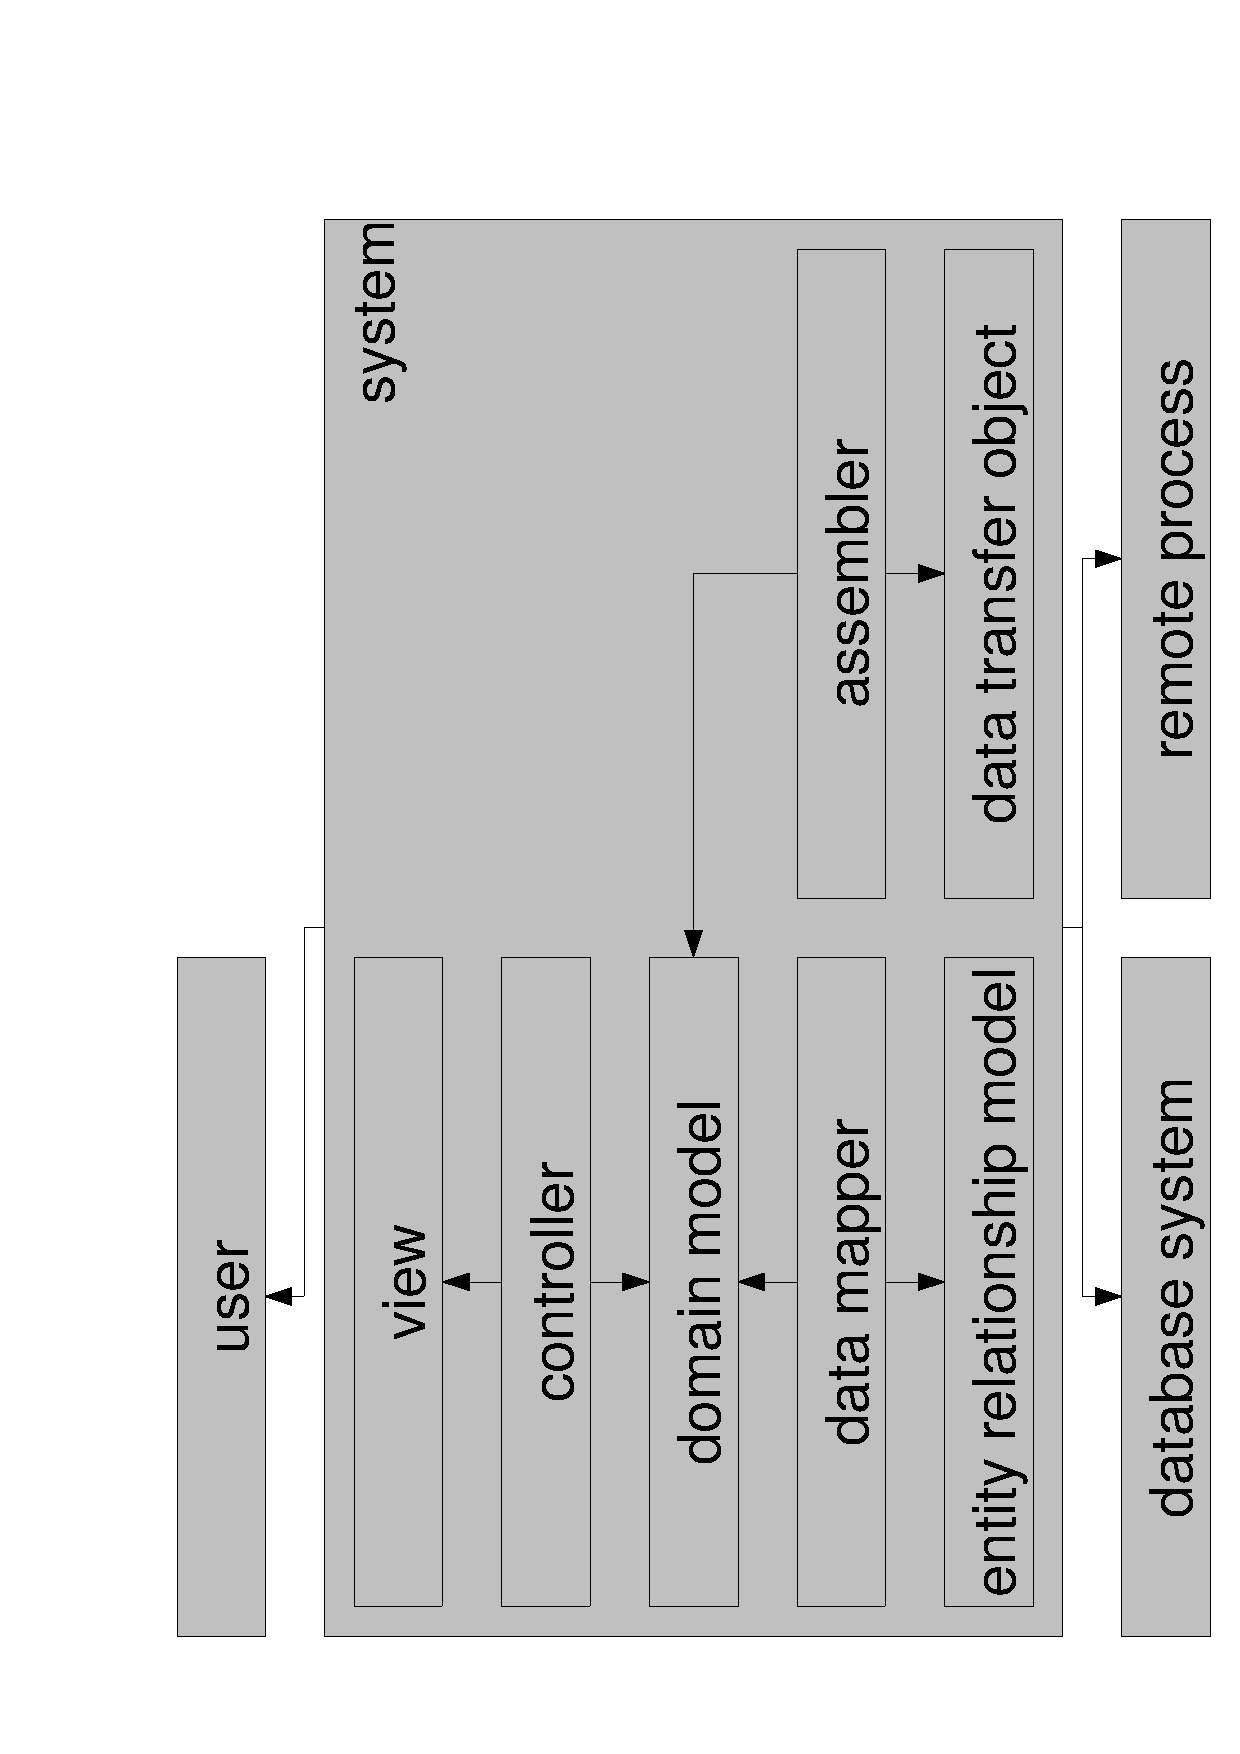
\includegraphics[scale=0.3,angle=-90]{graphic/placement.pdf}
        \caption{Communication Patterns placed in Layered Architecture}
        \label{placement_figure}
    \end{center}
\end{figure}

It is not difficult to figure out where the communication patterns of section
\ref{basic_patterns_heading} fit in here (figure \ref{placement_figure}): The
\emph{Model View Controller} (\emph{Presentation Layer}) determines the parts
to interact with a human user via the \emph{View}; the \emph{Data Mapper}
pattern with its inherent \emph{Entity Relationship Model} (ERM) encapsulates
mechanisms to connect to a persistence medium such as a \emph{Database} (DB);
the \emph{Data Transfer Object} (DTO) and its corresponding assemblers,
finally, serve as means of communication with remote servers.
